% !TeX spellcheck = en_GB
% !TeX encoding = UTF-8
% !TeX program = xelatex
%----------------------------------------------------------------------------
\chapter{Background}
%----------------------------------------------------------------------------

\section{Graph Neural Networks}

	Many real life problems can be best modelled with graphs and these representations can code a lot of information if assessed correctly. By developing techniques that work to extract this information and extrapolate from it effectively, we can build powerful systems that can predict, classify and advise based on graph data.
	
	\begin{figure}[!h]
		\centering
		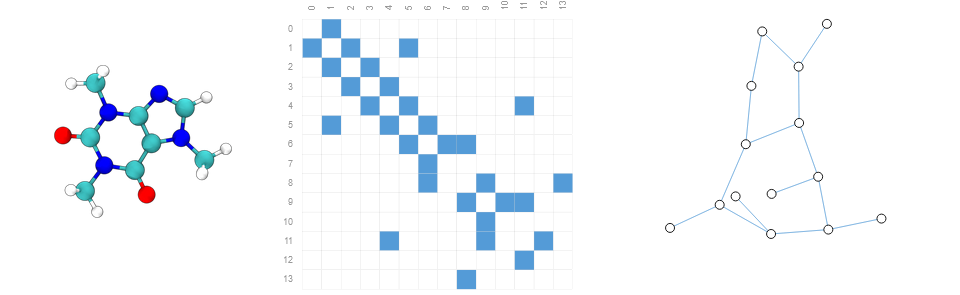
\includegraphics[width=\textwidth]{figures/molecule.png}
		\caption{From left to right: 3D representation of a caffeine molecule, its adjacency matrix, its graph representation. \cite{sanchez-lengeling2021a}}
	\end{figure}
	
	Graph algorithms have a long history in mathematics and there is a rich variety of graph related problems that are best solved using these classical discrete mathematical methods: pathfinding algorithms, breadth or depth-first search algorithms are used every day both in everyday IT applications and infrastructure, and also in research. But in certain cases these methods may not be well-equipped to handle the task at hand. With the large amount of data collected every day and the specialized tasks that need to be fulfilled there is reason to bring machine learning into graphs and the discipline has exploded in popularity in the last five years or so.

	\subsection{Neural Networks}
	
	Neural networks are an especially interesting and useful area of machine learning and data analysis: as referenced in their name, they were created in resemblance of the human brain's structure, mimicking the interconnected neurons. In recent years they became the flagship of AI research because of their ability to work on incredibly large datasets effectively and produce never seen before results. 
	
	The basis of a neural network are neurons which sum up incoming "signals" multiplied by weights and apply an activation function to their output. The network learns by updating these weights and biases based on the training data, to match the desired output to each piece of input. The activation function adds non-linearity to the model, making it capable of learning more complicated relationships in the data.
	
	Neurons are typically organized into layers in a neural network and the models usually benefit from having a large number of layers: modern models for more complex tasks can get very 'deep' which lead to the popularization of the term deep learning when talking about such models. But since having more layers makes a model more computationally intensive, leading to higher costs and slower inference, researchers are often looking to prune models or find architectures that deliver similar results while having a lower parameter count.
	
	Parameters in a model are updated through a process called backpropagation. Here, for labeled training data, the error of the prediction of the model is calculated through the use of a loss function. This should be representative of how far off the model was from the ground truth and also easy to work with derivation-wise and numerically. This is then "propagated back" through the model by deriving what each of the model's parameters contributed to this loss\ref{eq:backprop}. This is what's known as the gradient and it is used to perform gradient descent: based on the resulting derivative we have a direction to move in to lower the loss.
	
	\begin{align}
		\label{eq:backprop}
		\frac{\partial{E}}{\partial{w_{i,j}}} = \frac{\partial{E}}{\partial{o_j}}\frac{\partial{o_j}}{\partial{net_j}}\frac{\partial{net_j}}{\partial{w_{i,j}}},
	\end{align}
	
	
	In case of larger datasets it is impossible to calculate the gradient for the entire dataset in one go, so a process called stochastic gradient descent is used, where randomly selected subsets (batches) of the dataset are used to calculate it during training. Having a gradient, the other part needed is the learning rate: how much to change weight in the given direction. This can be considered hyperparameter of the model, but modern optimizers (such as ADAM) use adaptive learning rate optimization techniques (such as momentum and RMSProp) to adjust learning rate during training to ensure a smooth and fast convergence.
	
	%TODO cite
	From the most fundamental concepts of the original perceptron and the breakthrough idea of using backpropagation, neural networks became a widespread and varied phenomenon: there are architectures for different types of data optimized for different kinds of tasks; these models have proved to be applicable in almost any area.
	
	A very active and widely used branch of neural networks are convolutional neural networks (CNNs). These are most commonly used on image data and work by convolving learnable kernels with the input to extract features. This is useful for capturing spacial relationships allowing for better pattern detection while also greatly decreasing the number of trainable parameters compared to a fully connected feed-forward network. Attention-based networks are another important model class that became very successful in recent times. Transformer architectures are used in many disciplines and are capable of state-of-the-art results. Both of these concepts turn up in graph neural networks as well.
	%TODO esetleg ide a convolution, attention működéséről?
	
	\begin{figure}[!h]
		\centering
		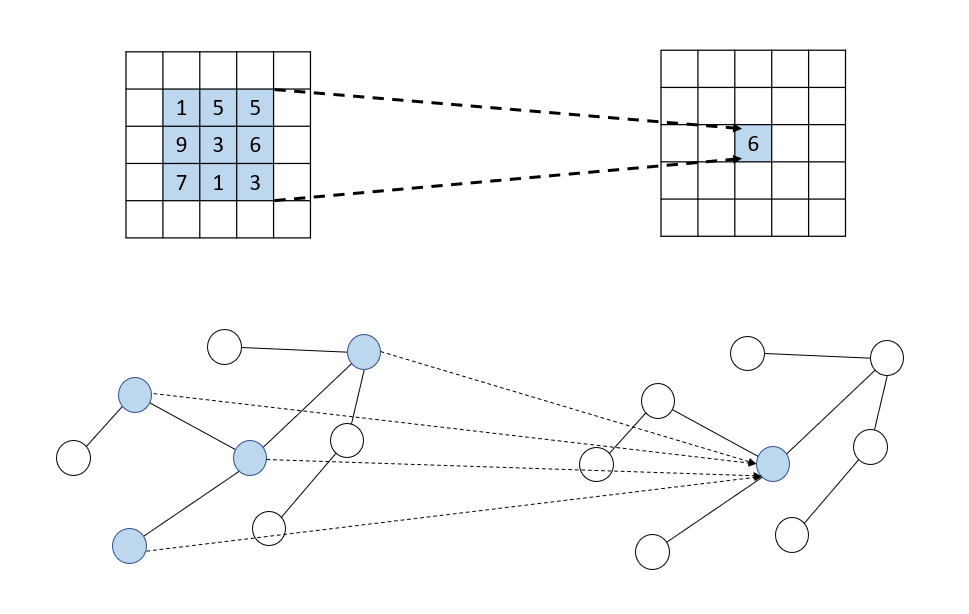
\includegraphics[width=\textwidth]{figures/convolution.png}
		\caption{Convolution on images versus graphs.}
	\end{figure}
	
	\subsection{Working on Graph Data}
	
	Graphs are a very versatile mathematical concept because of the way they lend themselves very neatly as a generalization. They have great expressive power when it comes to describing relations, groups and things with a rich inner structure. We can find graph-based datasets in a variety of domains: molecules in chemistry, interaction graphs in social sciences, knowledge graphs and computer networks. The level of abstraction they provide makes them suitable for use in many fields, as connections between items or molecules or people are vital in understanding complex natural systems.
	
	One area that is particularly rich with such examples is biology and medicine. Interactions between drugs, relationships between species and contact tracing in epidemiology are all important facets that can benefit from the ability to analyse graph datasets. We can also find interesting networks to analyse inside of organisms: the focus of this thesis is the analysis of network formed by brain regions and the interactions that happen in the human brain.
	
	Graphs are mathematically defined as a set of nodes (or vertices) and edges (or links) which run between two nodes. They can be categorized by their edge structure: directed graphs specifically code the information of a starting and end node, while undirected graphs do not. In terms of graph neural networks this is a very important distinction as it fundamentally alters how the network's meaning. Certain types of networks are designed with a specific type of graph in mind and might need special normalisation.
	
	Certain types of graphs with special properties can be especially interesting in certain areas. Trees (which contain no cycles) can be useful for describing containment hierarchies or sentence structures, for example. Based on semantic meaning we can also talk about heterogeneous graphs were nodes may represent entirely different things, purchase or interaction graphs in a recommender system where a vertex could be a user or an item to be purchased. In this case it is important to make this information available to the network.
	
	A graph dataset often codes much more information then just the mathematical structure itself. Ideally some information is available of each node; a feature descriptor vector for each node supplies more information for the network and also helps identify the node it is attached to: since graphs are order agnostic the model needs another way to identify which node is which. 
	
	The contents of such a descriptor vector must be domain specific. For example in case of a social network it would code information about a given person: age, gender, height. In case of a molecule prediction scenario it could be atomic weight or covalent radius. For the brain fMRI analysis case most relevant to this thesis, it could be information about a given brain region, average activation or even an activation timeseries.
	
	In case there is no suitable information available for the node feature vectors it is common practice to use rows of the identity matrix: in absence of additional data this can be useful to serve as the identification tool the network needs. In some cases information might be available in other ways, for example as edge weights or edge feature vectors. These could be descriptive of the users' interactions in a social network example.
	
	Node feature vectors can be concatenated together to form a matrix and together with the adjacency matrix (or edge weight matrix) of the graph they form a very neat representation of the graph. This makes the highly variable structure of the graph containable within a constant, well-structured manner that is crucial for machine learning applications.
	
	But since graphs can be used to represent complex structures and hierarchies, where this inner construction is more pronounced and relevant then in other cases, they require specialized methods when it comes to machine learning and neural networks. A lot of these methods take after image recognition or object detection solutions.
	
	The reason for this is that while images do not have explicitly structured data in the same way as graphs do, their contents can be in complex spatial relations with each other. A computer vision model needs to take these into account when performing complex tasks such as segmentation or creating a full description of what is happening in a photo. Even for simple object detection, more complex object have hierarchical structures that the model needs to 'understand' in some way.
	
		
	\subsubsection{Common tasks}
	\label{section:common_tasks}
	
	The motivation behind working with graph datasets is of course to perform some sort of inference using the patterns extracted from the training data. Since these datasets are diverse both in semantics and in structure this could mean a lot of different types of tasks. In this section the most common of these will be described with examples and commonly used methods for solving them.
	
	Most graph architectures work by assigning a vector to each node on their output. This is often called a node embedding: an $n$-dimensional vector is attached to the node that attempts to convey all available information about the node and its role in the graph structure, effectively embedding it in an $n$-dimensional space. Node embeddings are not strictly only generated in deep learning models, there are for example random-walk based methods for this purpose, such as node2vec. 
	
	\begin{figure}[!h]
		\centering
		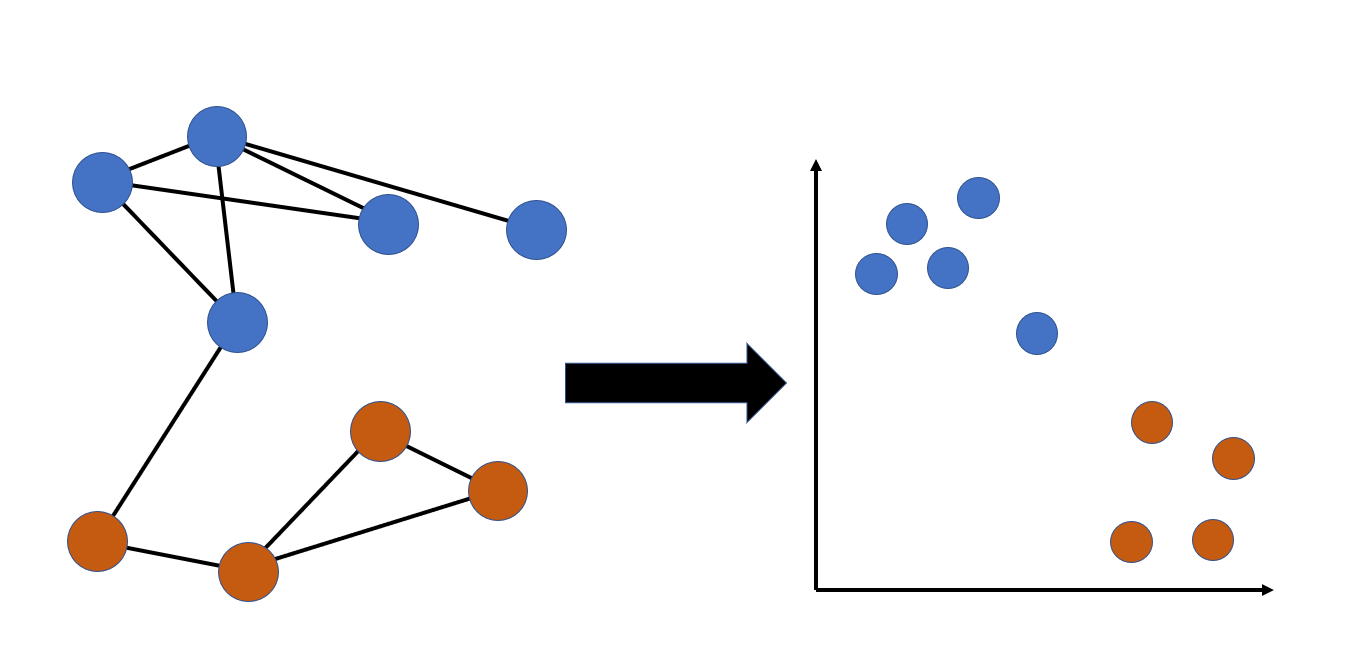
\includegraphics[width=\textwidth]{figures/embedding.png}
		\caption{Visual representation of node embeddings in 2 dimensional space.}
		\label{fig:embedding}
	\end{figure}
	
	In case of deep learning models the creation of node embedding is an iterative process as there is a new vector attached to the node after every layer. In this process the original feature vectors can be thought of as a sort of 0th iteration of the embedding, purely representing information about the node itself. With more and more layers aggregating information on a larger and larger neighbourhood of a node this slowly transforms into containing information of the structure of the network as well.
	
	%TODO find examples for these with citations
	
	\textbf{Node prediction.} In this type of task the goal is to infer some information about individual nodes of the graph. This could be sorting into already existing categories, classification or estimating a value related to the node, regression. Both types of tasks can work with datasets that are either graphs made up of labeled nodes that have a certain number of missing values or with training graphs that have fully labeled nodes, performing inference on graphs the model has not seen before. The second type of task is much more difficult, meaning models often performs significantly worse on such tasks, but oftentimes this reflects the real world scenarios and use-cases for models better.
	
	Since the network output is representative of a node and its role in the structure in the first place, this is the most straightforward type of task to solve using a deep learning model. In case of node classification a commonly used technique is to match the dimensions of the final embedding to the number of possible classes and have each of the values represent probability of class membership: this can work for both multi-label and simple classification using different activation functions.
	
	Another technique is to use a small fully connected MLP on the embedding for prediction. This is also useful in case of regression and gives a bit more control over the possible output formats. 
	
	\textbf{Graph prediction.} In case of this task the goal is to predict some sort of information about the entire graph. Node embeddings can be aggregated in a lot of ways to predict graph classes or labels. These aggregation methods are commonly referred to as a 'readout function': the values attached to nodes are 'read' together to reveal information about the entire graph.
	
	More common, basic readout methods are similar to the simpler pooling methods used in CNNs: node features can be averaged, summed or there can be a minimum or maximum choosing operation. 
	
	\textbf{Edge prediction.} There are two main types of edge prediction: either, similarly to nodes there is a specific feature or classification of edges we want to predict or the goal is to find edges in the graph that are not present in the structure right now but are most likely to exist; the second type is a very common task in recommender systems.
	
	There are multiple commonly used techniques for edge predictions using node embeddings generated by a GNN there are capable of providing either continuos or binary results. These methods usually rely on using the information about a pair of nodes to determine their 'compatibility' or other feature of their shared edge.
	
	\textbf{Clustering, influence prediction.} Clustering in this domain usually refers to clustering the nodes of the graph to find groups more 'similar' or 'closely connected'. There are a lot of classical solutions for this problem as well such as the Girvan-Newman algorithm which optimises an edge-betweenness metric and the Louvain method with uses modularity. 
	
	In case a GNN is used in this task it is in an unsupervised or semi-supervised manner, where it used to generate embeddings and then the embedding are clustered using a common clustering ML solution such as K-means or DBSCAN. Hybrid solutions are also possible: a neural network could be used to create edge weights that a classical algorithm could incorporate.
	
	Influence prediction is also an unsupervised task that seeks to find a node or multiple nodes that have the most influential role in the graph, finding hotspots of activity
	
	\subsubsection{Graph convolutions}
	
	The Laplacian of a graph is a square matrix $n \times n$ in size (where $n$ is the number of nodes in the graph). It can be calculated from the adjacency matrix and diagonal node degree matrix:
	
	$$ L = D - A, $$
	
	where L is the Laplacian, D is the diagonal node degree matrix and A is the adjacency matrix. In the diagonal node degree matrix there is similar to an identity matrix but in each row the instead of one we have the degree of the node corresponding to said row. The Laplacian can be used to build polynomials that can be used on node features.
	
	$$ p_w = w_0 I_n + w_1 L + w_2 L^2 + \cdots + w_d L^d = \sum_{i=0}^{d} w_i L^î $$
	
	These polynomials can be thought of as analogues of 'filters' in CNNs, and the coefficients $w_i$ as the weights of the ‘filters’. There exists a type of network that built directly on the concept of Laplacian polynomials: ChebNet used Chebyshev polynomials and normalized Laplacians to create a more numerically stable and 'stackable'.
	
	\begin{figure}[!h]
		\centering
		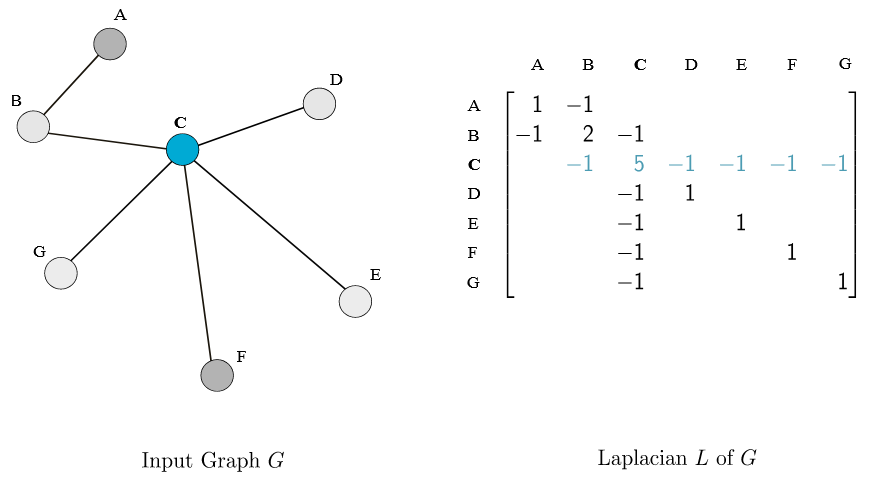
\includegraphics[width=0.9\textwidth]{figures/Laplacian.png}
		\caption{The Laplacian $L$ for an undirected graph $G$, with the row corresponding to node $C$ highlighted. Zeros in $L$ are not displayed above. The Laplacian $L$ depends only on the structure of the graph $G$, not on any node features. \cite{daigavane2021understanding}}
	\end{figure}
	
	ChebNet was a big step in ushering research into graph networks, as it motivated many to think about graph convolutions from a different perspective. Current graph neural networks utilize graph convolutions in ways that make use of 'computational shortcuts': bypassing costly operations such as eigenvalue calculations can make a model much more scalable, both in terms of data throughput and model size.
	
	These shortcuts often mean calculating local approximations of the graph convolutions. Local graph operations are often so called 'message passing' operations: every node in the graph sends a 'message' to its neighbours based on its own data and then each node aggregates the received messages. In practice this means each node vector is updated in a layer based on its neighbours.
	
	\begin{figure}[!h]
		\centering
		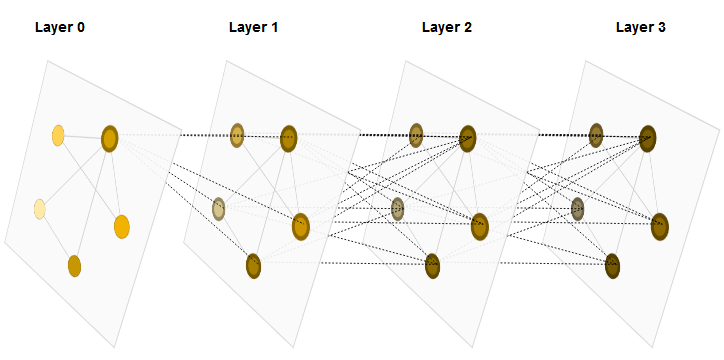
\includegraphics[width=\textwidth]{figures/gnn.png}
		\caption{Visualization of a GNN accumulating information via message passing. \cite{sanchez-lengeling2021a}}
	\end{figure}
		
	\subsection{Graph Neural Network Types}
	
	There are many architectures that fall under the umbrella of graph neural networks and they can be grouped by many different criteria with interesting similarities between them. In \cite{gnn_review} the authors break down the most common parts of graph architectures: a way of \textbf{propagating} information between nodes, a way of \textbf{sampling} relevant nodes when graphs and neighbourhoods get large, and, in case it is needed for the task at hand, a way of \textbf{pooling} information to represent subgraphs or graphs.
	
	 \begin{figure}[!h]
	 	\centering
	 	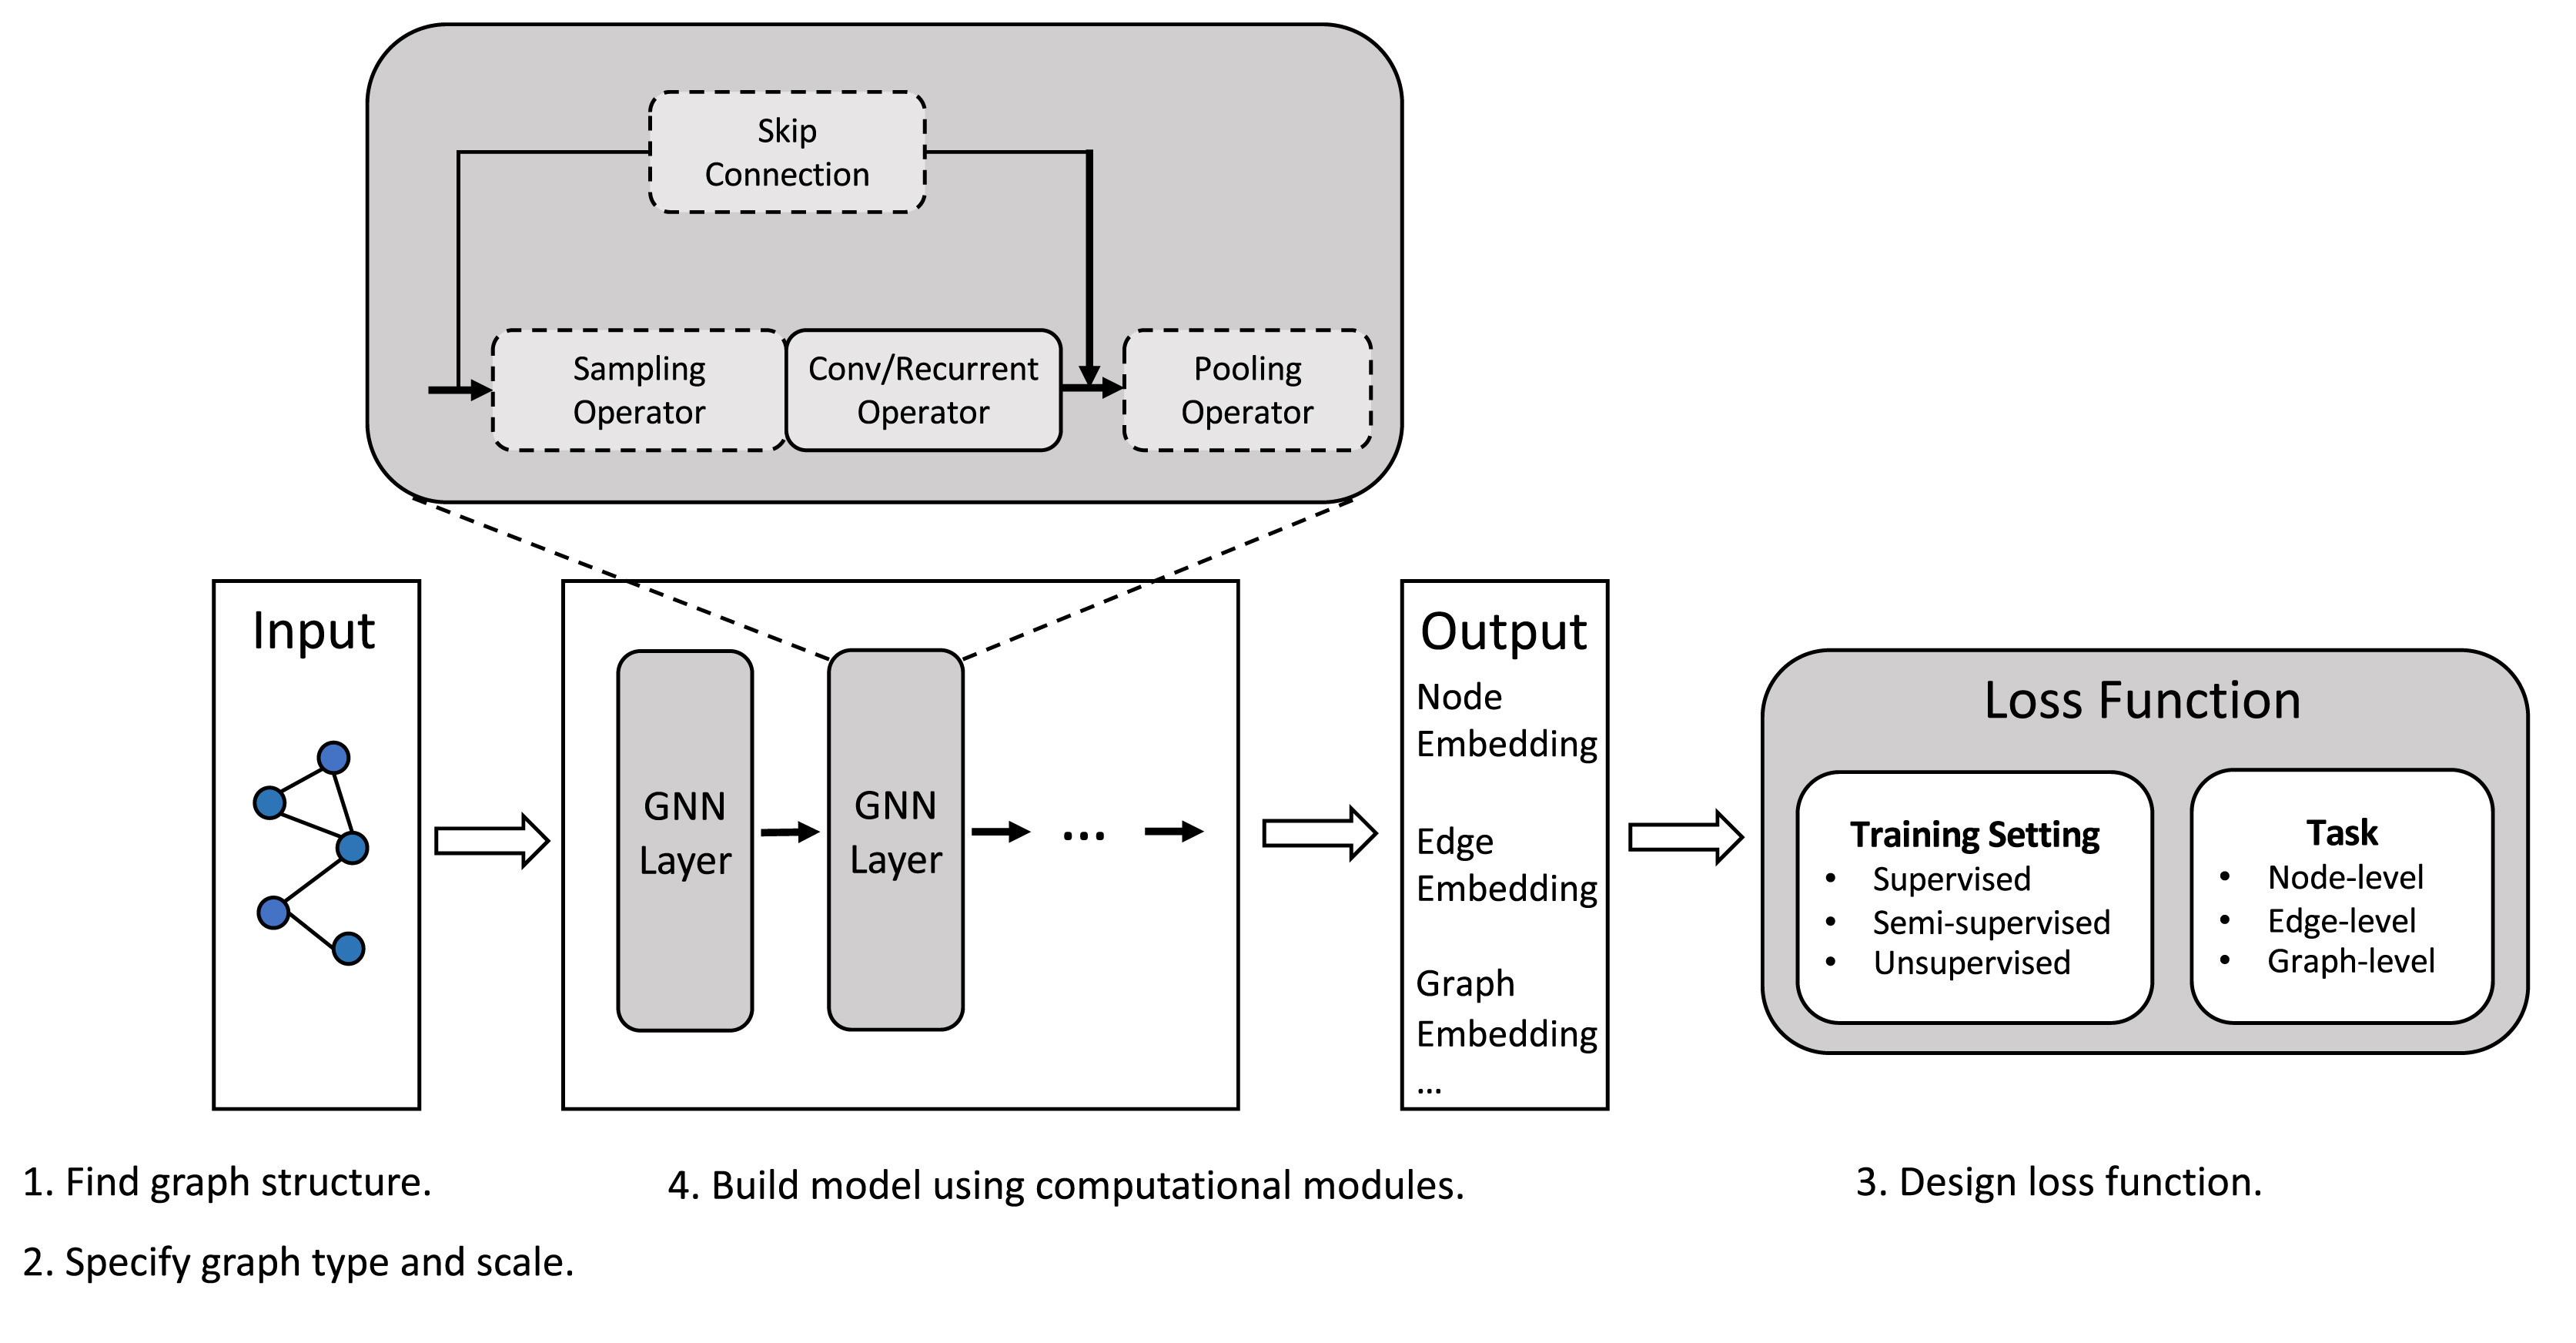
\includegraphics[width=\textwidth]{figures/gnn_general_structure.jpg}
	 	\caption{A generalized schematic of GNN architectures \cite{gnn_review}}
	 \end{figure}
	 
	 We can also differentiate architectures based on the type of graphs they operate on, the previously discussed task of the network\ref{section:common_tasks} or the used learning type: supervised (using labeled data), semi-supervised (using a small amount of labeled data to guide training) and unsupervised (using unlabeled data to find patterns).
	 
	 The most commonly used network types/layer types include GCNs (Graph Convolutional Network), GATs (Graph Attention Network), GraphSAGE (Graph Sample and AGgregatE). These are all convolution-based solutions with different approaches to the implementation. GCNs try to stay true to spectral convolutions following ChebNet's footsteps, GATs leverage the very powerful concept of attention for convolutions and GraphSAGE focuses on building a good way to sample large neighbourhoods in large graphs.
	 
	 In the realm of convolution based models MPNNs (Message Passing Neural Network) can be seen as a generalization of the concept, extracting common features from other methods, serving as a framework that can instantiate any of those models. Other than convolutions another type of architecture that has been used in graph networks with success has been recurrent networks. 
	 
	 \begin{figure}[!h]
	 	\centering
	 	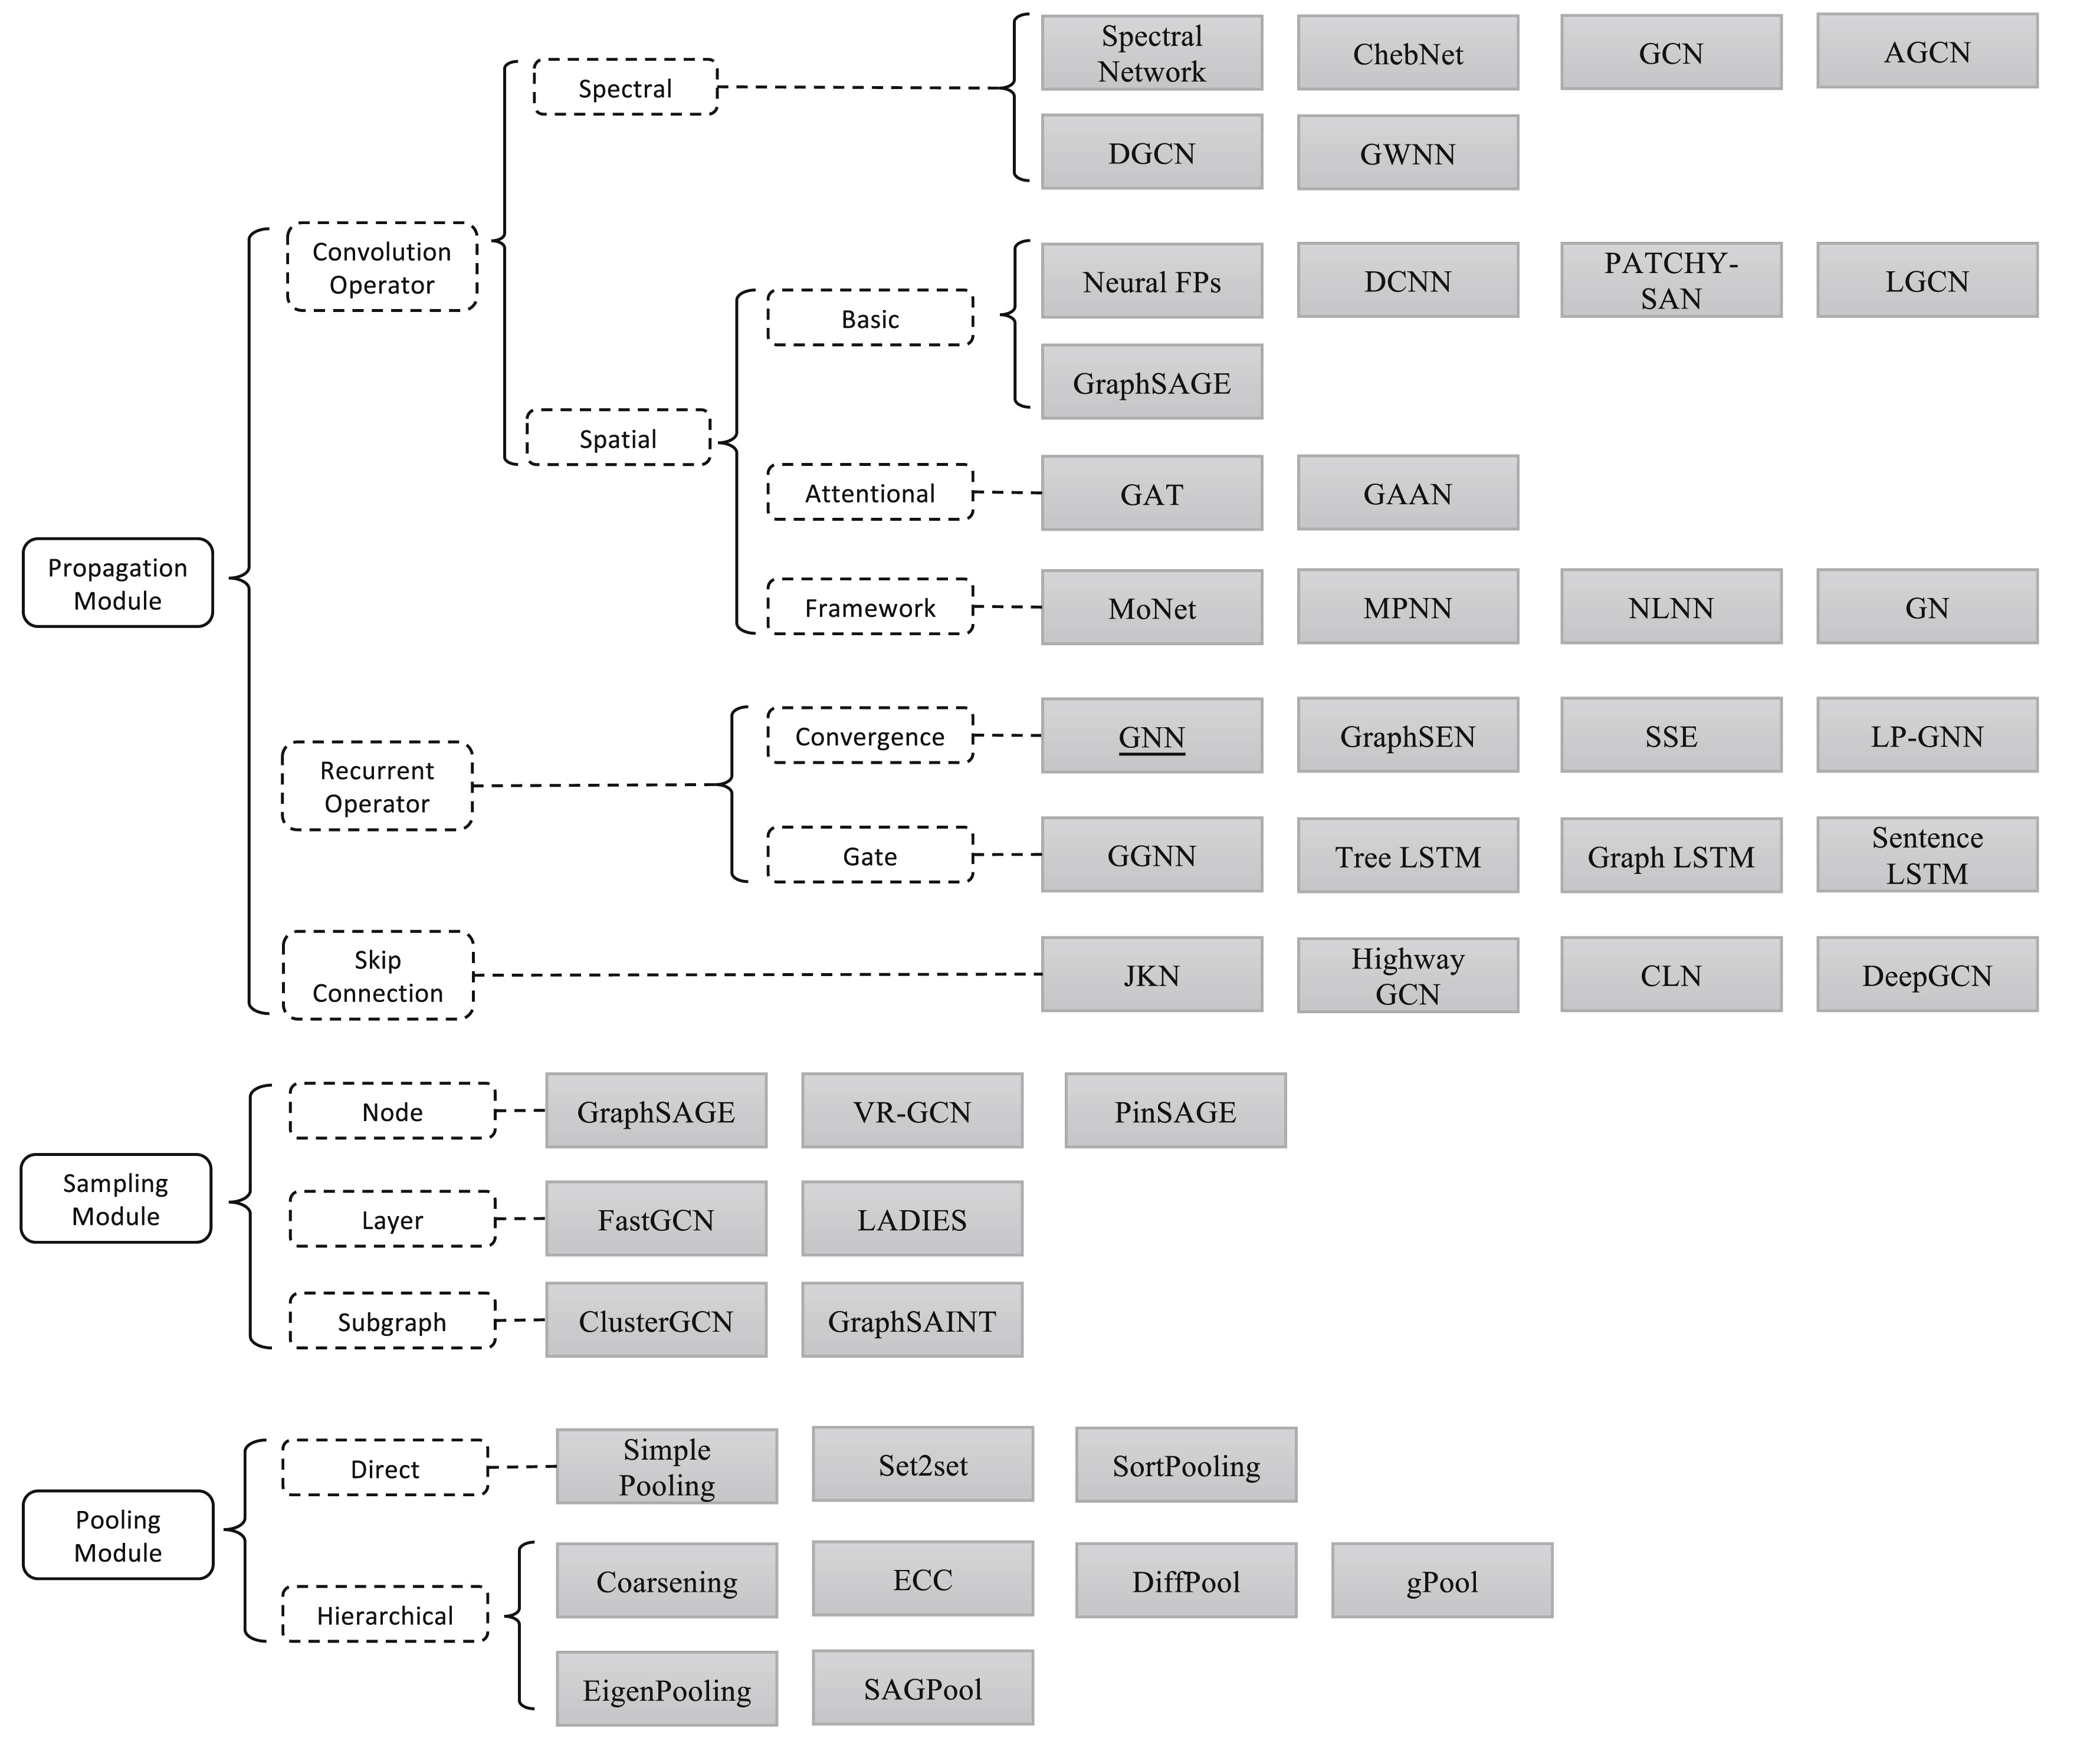
\includegraphics[width=\textwidth]{figures/gnn_types.jpg}
	 	\caption{GNN architectures grouped by characteristics\cite{gnn_review}}
	 \end{figure}
	
	\subsubsection{Graph Convolutional Networks}
	
	Graph Convolutional Networks (GCNs) expand on the idea of CNNs, which are commonly used in image processing. Observing from a graph perspective, an image can be considered a very special case of a graph, where pixels are nodes and their neighbours can be determined from the grid. This type of network generalizes the concept of local convolutions from the image domain to general graphs.
	
	\begin{align}
		H^{(l+1)} = f\left(H^{(l)}, A\right) = g\left(\hat{D}^{- \frac{1}{2}} \hat{A} \hat{D}^{- \frac{1}{2}} H^{(l)} W^{(l)}\right)
		\label{eq:layer}
	\end{align}
	
	Equation \ref{eq:layer} shows how the next layer's node feature vectors are calculated from the previous ones: $A$ is the adjacency matrix, $\hat{A}$ is the adjacency matrix with self-loops added in $(\hat{A} = A + I)$, $\hat{D}$ is the diagonal node degree matrix with the purpose of normalisation, $W$ is the learnable weight matrix and $g$ is some type of non-linear activation function, most commonly ReLU or leaky ReLU in practice.
	
	This computation model is a nice analogue for convolutions on images, and approximates spectral convolutions while remaining computationally stable and non-resource intensive. Layers can also be stacked nicely to allow information to travel further than the immediate neighbourhood of a node.
	
	\subsubsection{Graph Attention Networks}
	
	%TODO GATról írni kicsit
	
	
	\subsubsection{GraphSAGE}
	%TODO graphSAGEről is ha használom majd
	
	
\section{Medical data}

	We can call anything medical data that relates to human healthcare in one way or another. This most commonly means data collected by healthcare institutions about patients using sensor equipment, but it could also be information about a patient's habits or general environment, data from drug test trials or even location data in case of epidemiological contact tracing. 
	
	\subsection{Legal and ethical concerns}
	
	This kind of data is often very personal and regarded as sensitive data: people are entitled to equal treatment regardless of medical status and as such information about the health status of an individual is protected. Many patients do not want employers or other third parties who could use such information against them to know details about their conditions and their treatment.
	
	For this reason doctors are required to not give out patient information unless it is strictly necessary and/or they have the informed consent of the person. This puts medical researchers in an interesting position; medical researchers using machine learning even more so. Data collected specifically for experiments where subjects can consent to their data being used is a straightforward situation, but there is data collected every day, worldwide in hospitals that could be very useful for furthering medicine, but doing so poses data privacy concerns. This is especially important in case of machine learning and neural network research as these disciplines require a very large amount of data that is very hard to collect using only organized experiments.
	
	Developments in IT have lead to concerns about the effectiveness of data protection laws and in the European Union, for the sake of a more consistent and comprehensive protection of personal data, a General Data Protection Regulation (GDPR) has been enacted\cite{GDPR2016a}. There are fears that the combination of strict requirements and very limited research exemptions will stifle and severely restrict medical research, and that the current consent or anonymise approach is not suitable for data-intensive research\cite{mostert2016big}. 
	
	On the consent side of the equation, there is great difficulty in obtaining consent for personal data to be available for linkage, re-use and analysis for largely undetermined future research purposes\cite{anderson2015collection}. It is a question whether meaningful or freely given and informed consent can be given at the time of data collection as it may not be possible to foresee or comprehend the possible consequences of consenting: a person consenting to a DNA sample has no way of knowing what could be determined from their sample in 10 years time.
	
	Since personal data is defined as data that can directly or indirectly identify the individual\cite{personal}, the act of anonymisation seeks to remove identifiers that link datapoints to specific individuals to make the data suitable for use in research without infringing any of the patients' rights. A simple deletion of the name and address of the subject are usually not enough, as other characteristics can be enough to identify an individual. A commonly used technique is pseudonymisation where identifiers are removed and replaced with a unique keycode, but this is not truly anonymous as someone with the requisite key can link it back to the individual\cite{dataprot}. 
	
	Anonymisation requires extensive stripping of datasets and makes data linkage and update impossible in almost all scenarios, which makes datasets much less useful for research networks and projects. In addition to this, even in anonymised datasets there can be information that could negatively affect groups and lead to discrimination and stigmatisation\cite{mittelstadt2016ethics}.
	
	There is currently new EU regulations underway for the construction of a European Health Data Space Regulation (EHDS), which aims to establish a common framework for the use and exchange of health data across the EU\cite{ehds}. This seeks to empower individuals to be in charge of their medical data and to enable secure and trustworthy reuse for research and innovation.
	
	\subsection{Types of medical data}
	
	We can organize most medical/healthcare data into 7 categories that have differing use-cases and are of different interest to researchers\cite{healthcaredata}. Electronic Health Records (EHR) encompass the digital version of a patient's chart in a doctor's office, containing medical and treatment histories, but take the concept a step further offering a comprehensive view of patient health. Administrative data is similarly collected at clinical offices, detailing admissions, home care and prescriptions.
	
	Claims data refers to the data that is transferred to the insurance provider (public or private) for coverage and compensation. This contains information about procedures and tests as well as costs. Patient/disease registries help collect secondary data associated specifically with patients who share a particular diagnosis. These are particularly important for chronic conditions such as cancer or diabetes.
	
	Health surveys are conducted in the general population to assess the health of the population and estimate the prevalence of certain diseases. Clinical trial data refers to data collected in experiments and studies specifically for the purpose of research. Genomic data involves the molecular sequence in an organism’s genes, the role of each gene, the regulatory elements managing gene expression, and the connections among various genes.
	
	All of these types of data have their place in healthcare research and they occasionally overlap in their subjects, but they generally fall under different providers and legal protections. The data types most commonly used in machine learning and big data applications are EHRs, aggregated clinical trial data, administrative data, genomic data\cite{mostert2016big} and medical imaging data\cite{suzuki2017overview}.
	

	\subsection{Medical imaging}
	
	Non-invasive medical imaging techniques, such as MRI, X-ray, and CT scans, are essential tools in medicine, allowing physicians to understand the internal structures and functions of the body without the need for surgery. These techniques are invaluable for their ability to produce high-resolution images of different types of tissues, making it ideal for assessing the state and function of internal organs\cite{kasban2015comparative}.
	
	These techniques vary by advantages, disadvantages, risks, image quality, safety, costs and applications. Choosing the right technique for the examination of a particular patient or for data collection in an experiment is delicate balancing act that requires a physician well-versed in the particular niche.
	
	The basic concept for a medical imaging system consists of a source of energy that can penetrate the human body and as the energy passes through the body it is absorbed or deflected at varying levels according to the density and structure of tissues and organs. The energy is then detected by special detectors compatible with the energy source and the signals are then converted into images using the correct algorithm matching the system. Techniques are often categorized based on the type of energy passing through the body.
	
	The earliest discovered medical imaging tool was the X-ray, discovered by Röntgen in 1985, followed by the CT imaging technique in 1963. Research into the MRI started in the 1970s and the first prototypes were tested in 1980.
	
	
	%TODO ábra + esetleg egyéb képek
	
	%TODO kéne többet írni a röntgen + CT vonalról?
	
	\subsection{MRI and fMRI imaging}
	
	Magnetic Resonance Imaging (MRI) is a diagnostic technology that uses magnetic and radio frequency fields to image tissues\cite{atkins2002fully}. It produces high-fidelity images, while using no ionizing radiation, making possible its repeated use in patients. 
	
	\begin{figure}[!h]
		\centering
		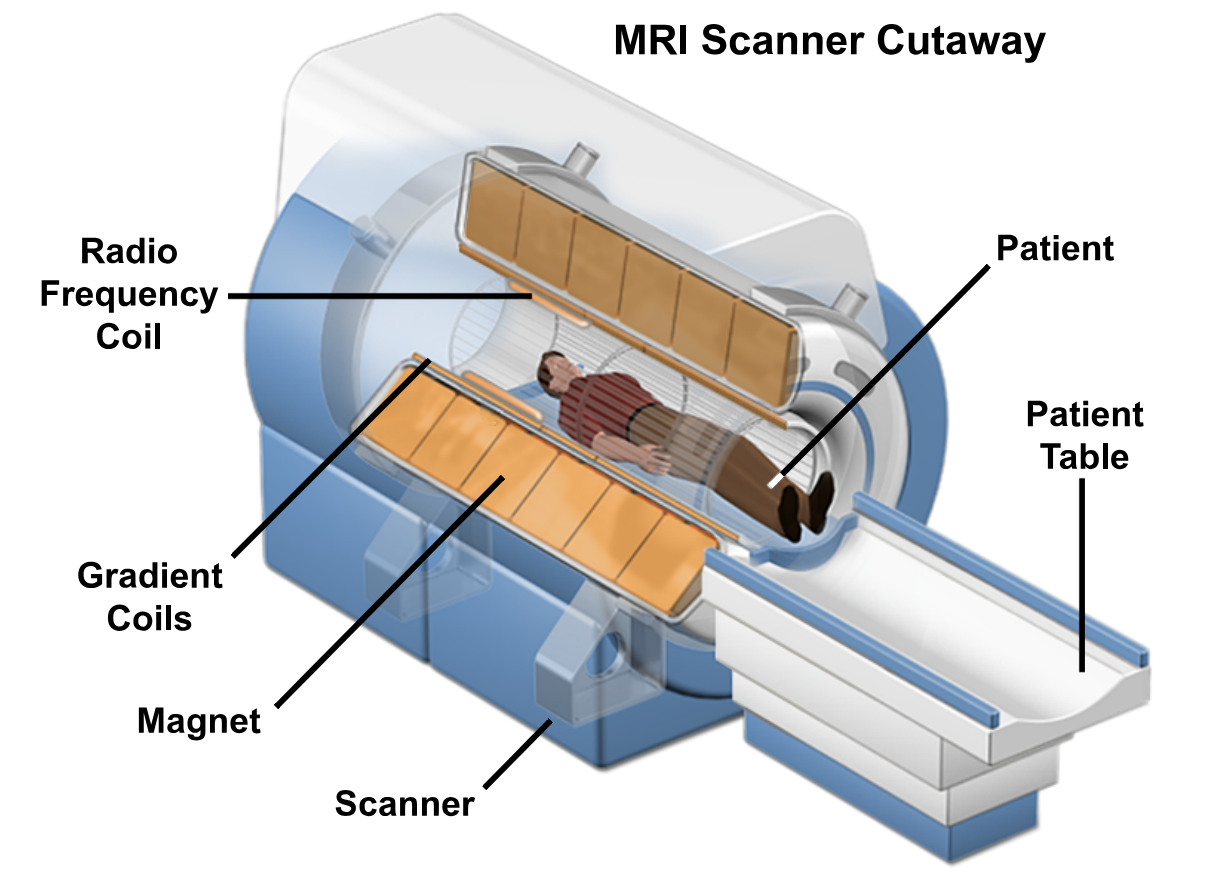
\includegraphics[width=\textwidth]{figures/mri_scanner.png}
		\caption{Schematic of an MRI machine\cite{mripage}}
	\end{figure}
	
	The procedure can be performed without contrast (no possible allergy problems) and is painless, but due to the long scan time and the design of machines it can induce claustrophobia and young children might require sedation to remain still. Comparatively to other imaging techniques MRI is also rather expensive, which is an important factor in deep learning applications where a large volume of data is needed.
	
	MRI is well suited for examining abdominal organs, such as the liver, joints and finding tumours, cysts and other abnormalities and unhealthy tissue in various parts of the body. It is also good for providing a view of the cranium and examining the brain and the spinal cord.
	
	\begin{figure}[!h]
		\centering
		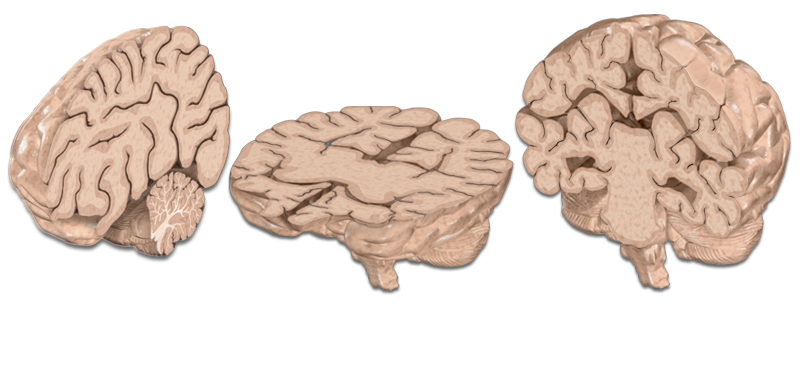
\includegraphics[width=\textwidth]{figures/slice_types.png}
		\caption{Types of slices in brain MRIs\cite{mripage}}
	\end{figure}
	
	Functional MRI (fMRI) extends the capabilities of MRI by measuring brain activity, via a method called Blood Oxygen Level Dependant Constant\cite{glover2011overview}. This technique works because of the haemodynamic response: when a part of the brain is activated, blood flows the region (after an initial dip). The surge of oxygenated blood increases the ratio of oxygenated hemoglobin.
	
	Oxygenated hemoglobin has different magnetic properties than deoxygenated hemoglobin, which causes measurable changes in the magnetic field, thus changing the readings of the MRI in the activated region, thus allowing detection of neural activity. The ability to capture neural activity in a non-invasive way is incredibly valuable in both clinical and research settings.
	
	There are two main types of fMRI scans: resting state and task-based fMRI. Resting state is self explanatory: patients are asked to remain still and relax while the scan is taken. For task-based scans, patients are given some sort of stimulus: either a task to complete, such as imagining moving a part of their body (for examining motor function activity) or holding a conversation, or simply being shown an image or text. 
	
		\subsubsection{Clinical significance }
		
		
		
	
		\subsubsection{Technical background}
		
		MRI technology builds on the physical phenomenon known as Nuclear Magnetic Resonance. Certain atomic nuclei, when exposed to a strong magnetic field, align themselves with this field. The hydrogen atom also shares this property and is abundant in all parts of the human body. 
		
		The aligned nuclei can then be perturbed by a radio frequency signal, which causes them to absorb the energy of the signal and go out of alignment with the original field. The nuclei then start to precess, during which they emit the absorbed energy, which is unique in different types of tissues in the body\cite{plewes2012physics}.
		
		MRI machines provide a strong, constant magnetic field, then send short, localized pulses of radio frequency signals to cause the misalignment. As these atoms realign themselves the machine uses the signals emitted to construct a three dimensional image of the area, comprised of individual cuboid elements, called voxels, based on the measurements.
		
		%TODO ide signal detection meg ilyenek? Vagy az too much?
		
		The number and size of voxels reflects the quality of the scan and high-resolution images permit the detailed analysis of brain responses. fMRIs recorded this way reflect neural activity: the presented task increases local neuron activity, which in turn increases metabolic rate, which also means increased blood flow, which translates into an increased MRI signal. The time it takes for this process to occur also means that the changes in the fMRI are delayed compared to the stimuli of the patient by 1-2 seconds\cite{deyoe1994functional}.
		
		\begin{figure}[!h]
			\centering
			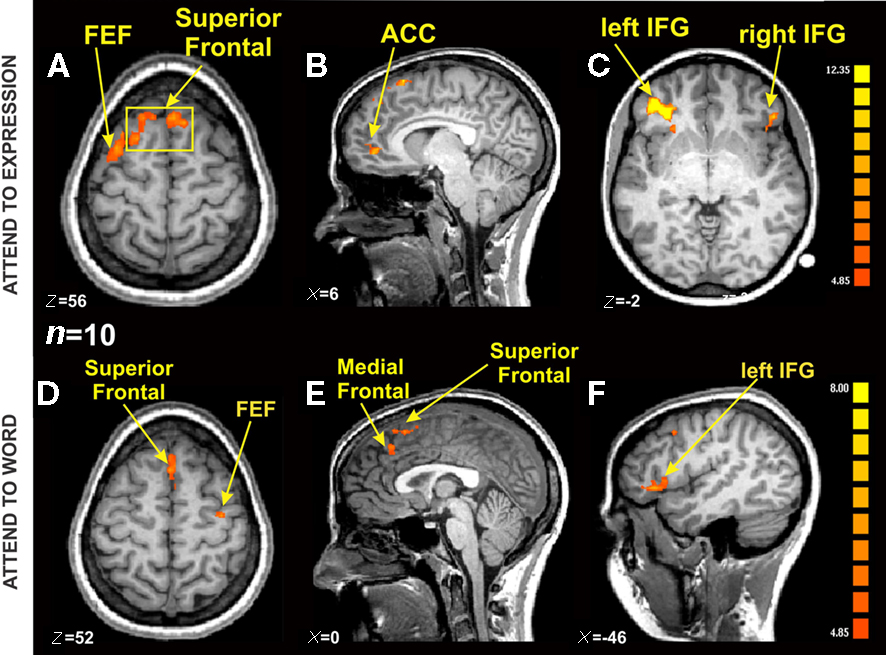
\includegraphics[width=\textwidth]{figures/fmri_example.jpg}
			\caption{Example of an fMRI scan showing different activations on expressions and speech\cite{ovaysikia2011word}}
		\end{figure}
		
		
		\subsubsection{Processing}
		
		An fMRI data set from a single session can either be thought of as $t$ volumes, one taken every few seconds, or as $v$ voxels, each with an associated time series of $t$ time points\cite{smith2004overview}. This raw four-dimensional data needs to be thoroughly preprocessed as a first step, before any meaningful conclusions can be drawn from it. The beginning of this procedure is very similar to other image or medical imaging preprocessing methods. There is however no consensus currently on the best methods for preprocessing fMRI data, so picking a strategy and parameters often works on a case-by-case basis, there are a few well-known pipelines that are available and commonly experimented with\cite{strother2006evaluating}.
		
		Despite their differences most pipelines accomplish most of the same few tasks: Slice-timing correction makes sure that when viewing a volume all of the voxels have been acquired at the same time, motion correction is applied to make sure each volume is aligned with every other one. Smoothing methods are applied to reduce noise and artifacts. Some methods also try to reduce variance in the scans by aligning them to a particular template.
		
		\subsubsection{ROIs and connectomes}
		
		For better analysis of the functional brain scans it is important to have a certain understanding of the functional areas of the brain to help understand the significance of certain regions firing. Brain atlases are sophisticated templates created by medical researchers as the average of many brains, giving a common coordinate system and also important information about the region at every voxel. With these atlases brain scans can be segmented into different functional centers which are commonly referred to as Regions of Interest (ROIs). 
		
		If the segmentation is completed for an entire scan, the average activation of these regions can be computed and used to draw conclusions about how this brain region works normally or how it participates in a given task. Even more information can be extracted if we are able to analyse how the regions interact with each other\cite{rogers2007assessing}. 
		
		The correlations between the fluctuations of activation in regions can reveal information about how these segments of the brain interact. These correlations change depending on the subject or the performed task, showing that regions interact differently under different conditions. Several methods have been proposed for assessing connectivity, most commonly using the time series of ROI activations to calculate covariance or correlation. 
		
		The goal is to yield a complete matrix of connectivity values between the regions, which can be thought of as sort of weighted brain graph describing how connected these regions are, often referred to as connectomes. A typical brain connectome is comprised of nodes for each brain ROI and edge weights that denote the connectivity strength between two ROIs\cite{bassett2017network}.
		
		